\documentclass[10pt]{article}
\usepackage[margin=1in]{geometry}
\usepackage{cite}
\usepackage{algorithm}
\usepackage{algpseudocode}
\usepackage{amsmath}
\usepackage{gensymb}
\usepackage{tensor}
\usepackage{amssymb}
\usepackage{graphics}
\usepackage{graphicx}
\usepackage{rotating}
\usepackage{verbatim}
\usepackage[caption=false,font=footnotesize,subrefformat=parens,labelformat=parens]
{subfig}
\graphicspath{{graphics/}}
\DeclareGraphicsExtensions{.png}
\title{\bf Assignment \#2
}

\author{\parbox{4 in}{\centering Introduction to Intelligent Robotic Systems}\\
  CSCI 5551\\ \\
  Daniel Koniar\\
  {\tt\small \{konia013\}@umn.edu}\\
}  

\begin{document}
\maketitle
\thispagestyle{empty}
\pagestyle{empty}

%%%%%%%%%%%%%%%%%%%%%%%%%%%%%%%%%%%%%%%%%%%%%%%%%%%%%%%%%%%%%%%%%%%%%%%%%%%%%%%%
\section*{Problem 1}
\subsection*{Exercise 4.2}
Derive the inverse kinematics of the three-link manipulator of Chapter 3, Exercise 3.3
\subsubsection*{\textit{\textbf{Step 1: Assign Frames}}}
\begin{figure}[!h]
\centering
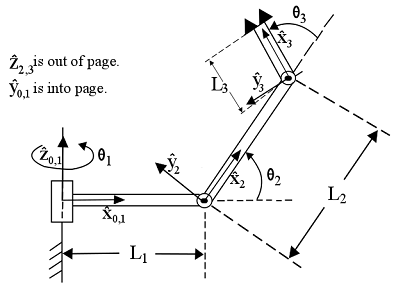
\includegraphics[]{Fig329}
\it{\caption{Frame assignment for Figure 3.29 (Exercise 3.3) on page 93\cite{textbook}}}
\end{figure}
\subsubsection*{\textit{\textbf{Step 2: Fill the D-H Table}}}
\begin{center}
\begin{tabular}{ l | c c c c }
  $i$ & $\alpha_{i-1}$ & $a_{i-1}$ & $d_{i}$ & $\theta_{i}$ \\
  \hline
  1   & $0$            & $0$       & $0$     & $\theta_{1}$\\ 
  2   & $90\degree$    & $L_{1}$   & $0$     & $\theta_{2}$\\
  3   & $0$            & $L_{2}$   & $0$     & $\theta_{3}$\\
\end{tabular}
\end{center}
\subsubsection*{\textit{\textbf{Step 3: }}$\bf{\it{\forall_{i}}}$ compute $\bf{\it{ \tensor*[^{i-1}_{i}]{T}{}}}$}
%%%%%%%%%%%%%%%%%%%%% BEGIN INITIAL SETUP %%%%%%%%%%%%%%%%%%%%%%%%%%%%%%%%%%%%%%%%%%
\[
\tensor*[^{0}_{1}]{T}{} =
\begin{bmatrix}
    c_{1}        & -s_{1}       & 0     & 0      \\
    s_{1}        & c_{1}        & 0     & 0      \\
    0            & 0            & 1     & 0      \\
    0            & 0            & 0     & 1
\end{bmatrix}, 
\tensor*[^{1}_{2}]{T}{} =
\begin{bmatrix}
    c_{2}        & -s_{2}       & 0     & L_{1}  \\
    0            & 0            & -1    & 0      \\
    s_{2}        & c_{2}        & 0     & 0      \\
    0            & 0            & 0     & 1
\end{bmatrix}, 
\tensor*[^{2}_{3}]{T}{} =
\begin{bmatrix}
    c_{3}        & -s_{3}       & 0     & L_{2}  \\
    s_{3}        & c_{3}        & 0     & 0      \\
    0            & 0            & 1     & 0      \\
    0            & 0            & 0     & 1
\end{bmatrix}\] \\
%%%%%%%%%%%%%%%%%%%%% COMPUTE 0 to 2 %%%%%%%%%%%%%%%%%%%%%%%%%%%%%%%%%%%%%%%%%%
\[
\tensor*[^{0}_{2}]{T}{} = 
\tensor*[^{0}_{1}]{T}{} \tensor*[^{1}_{2}]{T}{} = 
\begin{bmatrix}
    c_{1}        & -s_{1}       & 0     & 0      \\
    s_{1}        & c_{1}        & 0     & 0      \\
    0            & 0            & 1     & 0      \\
    0            & 0            & 0     & 1
\end{bmatrix}
\begin{bmatrix}
    c_{2}        & -s_{2}       & 0     & L_{1}  \\
    0            & 0            & -1    & 0      \\
    s_{2}        & c_{2}        & 0     & 0      \\
    0            & 0            & 0     & 1
\end{bmatrix} =
\begin{bmatrix}
    c_{12}       & -c_{1}s_{2}  & s_{1} & c_{1}L_{1}     \\
    s_{1}c_{2}   & -s_{12}      & -c_{1}& s_{1}L_{1}     \\
    s_{2}        & c_{2}        & 0     & 0      \\
    0            & 0            & 0     & 1
\end{bmatrix}
\] \\
%%%%%%%%%%%%%%%%%%%%% COMPUTE 0 to 3 %%%%%%%%%%%%%%%%%%%%%%%%%%%%%%%%%%%%%%%%%%
\[
\tensor*[^{0}_{3}]{T}{} = 
\tensor*[^{0}_{2}]{T}{} \tensor*[^{2}_{3}]{T}{} =
\begin{bmatrix}
    c_{12}       & -c_{1}s_{2}  & s_{1} & c_{1}L_{1}     \\
    s_{1}c_{2}   & -s_{12}      & -c_{1}& s_{1}L_{1}     \\
    s_{2}        & c_{2}        & 0     & 0      \\
    0            & 0            & 0     & 1
\end{bmatrix}
\begin{bmatrix}
    c_{3}        & -s_{3}       & 0     & L_{2}  \\
    s_{3}        & c_{3}        & 0     & 0      \\
    0            & 0            & 1     & 0      \\
    0            & 0            & 0     & 1
\end{bmatrix}
\]\\
\[
\tensor*[^{0}_{3}]{T}{} =
\begin{bmatrix}
c_{123}-c_{1}s_{2,3} & -c_{12}s_{3}-c_{13}s_{2}& s_{1} & c_{1}L_{1} + c_{12}L_{2}\\
s_{1}c_{23}-s_{123}    & -s_{13}c_{2}-s_{12}c_{3} & -c_{1}& s_{1}L_{1} + s_{1}c_{2}L_{2}\\
s_{2}c_{3}+c_{2}s_{3}  & c_{23}-s_{23}            & 0     & s_{2}L_{2}\\
0                      & 0                        & 0     & 1
\end{bmatrix}
\]
%%%%%%%%%%%%%%%%%%%%%%%%%%%%%%% COMPLETED AND CORRECT %%%%%%%%%%%%%%%%%%%%%%%%%%%%
\subsubsection*{\textbf{\textit{Step 4: Find }}$\bf{\it{\theta_{1}}}$, $\bf{\it{\theta_{2}}}$, $\bf{\it{\theta_{3}}}$}
First, Let:
\[
\begin{bmatrix}
c_{123}-c_{1}s_{23} & -c_{12}s_{3}-c_{13}s_{2}& s_{1} & c_{1}L_{1} + c_{12}L_{2}\\
s_{1}c_{23}-s_{123}    & -s_{13}c_{2}-s_{12}c_{3} & -c_{1}& s_{1}L_{1} + s_{1}c_{2}L_{2}\\
s_{2}c_{3}+c_{2}s_{3}  & c_{23}-s_{23}            & 0     & s_{2}L_{2}\\
0                      & 0                        & 0     & 1
\end{bmatrix} = 
\begin{bmatrix}
r_{11} & r_{12} & r_{13} & x\\
r_{21} & r_{22} & r_{23} & y\\
r_{33} & r_{32} & r_{33} & z\\
0      & 0      & 0      & 1
\end{bmatrix}
\]
Now, let us first solve for $\theta_{1}$ and to do so, let we will use $x$ and $y$ from the matrix above to produce the following:
\[\dfrac{y}{x} = 
\dfrac{s_{1}(L_{1} + c_{2}L_{2})}{c_{1}(L_{1} + c_{2}L_{2})} =
\dfrac{s_{1}}{c_{1}}\]

\[
\theta_{1} = {tan^{-1}}\bigg(\dfrac{y}{x}\bigg)\]
\[
s_{1} = \dfrac{y}{x\sqrt{1 + \bigg(\dfrac{y}{x}\bigg)^2}} =
\dfrac{y}{\sqrt{x^2 + y^2}}, \mbox{     }
c_{1} = \dfrac{1}{\sqrt{1 + \bigg(\dfrac{y}{x}\bigg)^2}} =
\dfrac{x}{\sqrt{x^2 + y^2}}
\]
Now, let us solve for $\theta_{2}$.  For this, first lets solve for $s_{2}$, then for $c_{2}$:
\[z = s_{2}L_{2}\mbox{   } \Rightarrow \mbox{   }
s_{2} = \dfrac{z}{L_2}, \mbox{    }
c_{2} = \sqrt{1-{s_{2}}^{2}} = 
\sqrt{1-\bigg(\dfrac{z}{L_2}\bigg)^{2}} =
\dfrac{\sqrt{L_{2}^2 - z^2}}{L_2}
\]
\[
\theta_{2} = tan^{-1}\bigg(\dfrac{s_{2}}{c_{2}}\bigg) =
tan^{-1}\Bigg(\dfrac{\dfrac{z}{L_2}}{\dfrac{\sqrt{L_{2}^2 - z^2}}{L_2}}\Bigg) =
tan^{-1}\bigg(\dfrac{z}{\sqrt{L_{2}^2 - z^2}}\bigg)
\]
Lastly, we will solve $\theta_{3}$ by using the sum of angles formula as such:
\[
\dfrac{r_{33}}{r_{32}} = \dfrac{s_{2}c_{3}+c_{2}s_{3}}{c_{23}-s_{23}} =
\dfrac{s(\theta_{2} + \theta_{3})}{c(\theta_{2} + \theta_{3})}
\]
\[
\theta_{2} + \theta_{3} = tan^{-1}\bigg(\dfrac{r_{33}}{r_{32}}\bigg) 
\mbox{     } \Rightarrow \mbox{      } 
\theta_{3} = tan^{-1}\bigg(\dfrac{r_{33}}{r_{32}}\bigg) - \theta_{2}
\mbox{     } \Rightarrow \mbox{      }
\theta_{3} = tan^{-1}\bigg(\dfrac{r_{33}}{r_{32}}\bigg) - tan^{-1}\bigg(\dfrac{z}{\sqrt{L_{2}^2 - z^2}}\bigg)
\]
\subsection*{Exercise 4.4}
Derive the inverse kinematics of the 3-DOF manipulator of Chapter 3, Example 3.4
\subsubsection*{\textit{\textbf{Step 1: Assign Frames}}}
\begin{figure}[!h]
\centering
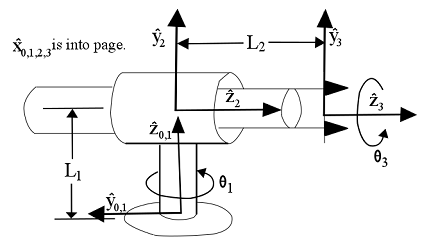
\includegraphics[]{Fig310}
\it{\caption{Frame assignment for Figure 3.10 (Example 3.4) on page 72\cite{textbook}}}
\end{figure}
\subsubsection*{\textit{\textbf{Step 2: Fill the D-H Table}}}
\begin{center}
\begin{tabular}{ l | c c c c }
  $i$ & $\alpha_{i-1}$ & $a_{i-1}$ & $d_{i}$ & $\theta_{i}$\\
  \hline
  1   & $0$            & $0$       & $L_{1}$ & $\theta_{1}$\\ 
  2   & $90\degree$    & $0$       & $L_{2}$ & $0$         \\
  3   & $0$            & $0$       & $0$     & $\theta_{3}$\\
\end{tabular}
\end{center}
\subsubsection*{\textit{\textbf{Step 3: }}$\bf{\it{\forall_{i}}}$ compute $\bf{\it{ \tensor*[^{i-1}_{i}]{T}{}}}$}
%%%%%%%%%%%%%%%%%%%%% BEGIN INITIAL SETUP %%%%%%%%%%%%%%%%%%%%%%%%%%%%%%%%%%%%%%%%%%
\[
\tensor*[^{0}_{1}]{T}{} =
\begin{bmatrix}
    c_{1}        & -s_{1}       & 0     & 0      \\
    s_{1}        & c_{1}        & 0     & 0      \\
    0            & 0            & 1     & L_{1}  \\
    0            & 0            & 0     & 1
\end{bmatrix}, 
\tensor*[^{1}_{2}]{T}{} =
\begin{bmatrix}
    1            & 0            & 0     & 0      \\
    0            & 0            & -1    & -L_{2} \\
    0            & 1            & 0     & 0      \\
    0            & 0            & 0     & 1
\end{bmatrix}, 
\tensor*[^{2}_{3}]{T}{} =
\begin{bmatrix}
    c_{3}        & -s_{3}       & 0     & 0      \\
    s_{3}        & c_{3}        & 0     & 0      \\
    0            & 0            & 1     & 0      \\
    0            & 0            & 0     & 1
\end{bmatrix}\] \\
%%%%%%%%%%%%%%%%%%%%% COMPUTE 0 to 2 %%%%%%%%%%%%%%%%%%%%%%%%%%%%%%%%%%%%%%%%%%
\[
\tensor*[^{0}_{2}]{T}{} = 
\tensor*[^{0}_{1}]{T}{} \tensor*[^{1}_{2}]{T}{} = 
\begin{bmatrix}
    c_{1}        & -s_{1}       & 0     & 0      \\
    s_{1}        & c_{1}        & 0     & 0      \\
    0            & 0            & 1     & L_{1}  \\
    0            & 0            & 0     & 1
\end{bmatrix}
\begin{bmatrix}
    1            & 0            & 0     & 0      \\
    0            & 0            & -1    & -L_{2} \\
    0            & 1            & 0     & 0      \\
    0            & 0            & 0     & 1
\end{bmatrix} =
\begin{bmatrix}
    c_{1}        & 0            & s_{1} & s_{1}L_{2}    \\
    s_{1}        & 0            & -c_{1}& -c_{1}L_{2}   \\
    0            & 1            & 0     & L_{1}         \\
    0            & 0            & 0     & 1
\end{bmatrix}
\] \\
%%%%%%%%%%%%%%%%%%%%% COMPUTE 0 to 3 %%%%%%%%%%%%%%%%%%%%%%%%%%%%%%%%%%%%%%%%%%
\[
\tensor*[^{0}_{3}]{T}{} = 
\tensor*[^{0}_{2}]{T}{} \tensor*[^{2}_{3}]{T}{} =
\begin{bmatrix}
    c_{1}        & 0            & s_{1} & s_{1}L_{2}    \\
    s_{1}        & 0            & -c_{1}& -c_{1}L_{2}   \\
    0            & 1            & 0     & L_{1}         \\
    0            & 0            & 0     & 1
\end{bmatrix}
\begin{bmatrix}
    c_{3}        & -s_{3}       & 0     & 0      \\
    s_{3}        & c_{3}        & 0     & 0      \\
    0            & 0            & 1     & 0      \\
    0            & 0            & 0     & 1
\end{bmatrix} =
\begin{bmatrix}
c_{13}           & -c_{1}s_{3}  & s_{1} & s_{1}L_{2}  \\
s_{1}c_{3}       & -s_{13}      & -c_{1}& -c_{1}L_{2} \\
s_{3}            & c_{3}        & 0     & L_{1}       \\
0                & 0            & 0     & 1
\end{bmatrix}
\]
%%%%%%%%%%%%%%%%%%%%%%%%%%%%%%% COMPLETED AND CORRECT %%%%%%%%%%%%%%%%%%%%%%%%%%%%
\subsubsection*{\textbf{\textit{Step 4: Find }}$\bf{\it{\theta_{1}}}$, $\bf{\it{L_{2}}}$, $\bf{\it{\theta_{3}}}$}
First, Let:
\[
\begin{bmatrix}
c_{13}           & -c_{1}s_{3}  & s_{1} & s_{1}L_{2}  \\
s_{1}c_{3}       & -s_{13}      & -c_{1}& -c_{1}L_{2} \\
s_{3}            & c_{3}        & 0     & L_{1}       \\
0                & 0            & 0     & 1
\end{bmatrix} = 
\begin{bmatrix}
r_{11} & r_{12} & r_{13} & x\\
r_{21} & r_{22} & r_{23} & y\\
r_{33} & r_{32} & r_{33} & z\\
0      & 0      & 0      & 1
\end{bmatrix}
\]
Now, we can solve for $\theta_{1}$ using $x$ and $y$ within the matrix:
\[
\dfrac{x}{y} = \dfrac{s_{1}L_{2}}{-c_{1}L_{2}} = \dfrac{s_{1}}{-c_{1}}
\mbox{     }\Rightarrow\mbox{     }
\theta_{1} = {tan^{-1}}\bigg(\dfrac{x}{y}\bigg)
\]
\[
s_{1} = \dfrac{x}{y\sqrt{1 + \bigg(\dfrac{x}{y}\bigg)^2}} =
\dfrac{x}{\sqrt{x^2 + y^2}}, \mbox{     }
c_{1} = \dfrac{1}{\sqrt{1 + \bigg(\dfrac{x}{y}\bigg)^2}} =
\dfrac{y}{\sqrt{x^2 + y^2}}
\]
Next, we can solve for $L_{2}$ using part of what was computed for $s_{1}$ and putting it into the equation for $x$:
\[
x = s_{1}L_{2} \mbox{     }\Rightarrow\mbox{     }
L_{2} = \dfrac{x}{s_{1}} = \dfrac{x}{\dfrac{x}{\sqrt{x^2 + y^2}}}
= \sqrt{x^2 + y^2}
\]
Lastly, we can solve for $\theta_{3}$ with the following:
\[
\dfrac{r_{33}}{r_{32}} = \dfrac{s_{3}}{c_{3}} \mbox{     } \Rightarrow \mbox{      }\theta_{3} = tan^{-1}\bigg(\dfrac{r_{33}}{r_{32}}\bigg)
\]

%%%%%%%%%%%%%%%%%%%%%%%%%%%%%%%%%%%%%%%%%%%%%%%%%%%%%%%%%%%%%%%%%%%%%%%%%%%%%%%%
\section*{Problem 2}
\subsection*{Exercise 4.7}
Make a list of factors that might affect the repeatability of a manipulator. Make a second list of additional factors that affect the accuracy of a manipulator.
\begin{itemize}
\item Factors that might affect the repeatability of a manipulator are:
\begin{enumerate}
\item The motors encoders, which are used to convert the position into electrical signals.  These need to be consistent for repeatability.
\item The manipulator's rotational speed can affect repeatability if tasks are performed at different speeds.
\item The manipulator's build quality, where better parts can lead to better precision, which will help maintain a reasonable state of repeatability.
\end{enumerate}
\item Additional Factors that might affect the accuracy of a manipulator:
\begin{enumerate}
\item The speed at which the manipulator is moving can affect it's accuracy.  At certain velocities the manipulator can become unstable.
\item An uncalibrated manipulator would present loss of accuracy, but still possibly maintain repeatability.
\item The distance from the base frame of the robot to the end effector, where as it increases, accuracy decreases.  This is due to forces applying higher torque on the base frame as it reaches outward.
\end{enumerate}
\end{itemize}
\pagebreak
\section*{Problem 3} %%COMPLETE%%
\subsection*{Exercise 4.11}
A 2-DOF position table is used to orient parts for arc-welding.  The forward kinematics
that locate the bed of the table (link 2) with respect to the base (link 0) are
\[
\begin{bmatrix}
    c_{1} c_{2}  & -c_{1} s_{2} & s_{1} & l_{2} s_{1} + l_{1} \\
    s_{2}        & c_{2}        & 0     & 0 \\
    -s_{1} c_{2} & s_{1} s_{2}  & c_{1} & l_{2} c_{1} + h_{1} \\
    0            & 0            & 0     & 1
\end{bmatrix}
\]
Given any unit direction fixed in the frame of the bed (link 2), $\tensor*[^{2}]{\hat{V}}{}$, give the inverse-kinematic solution for $\theta_{1}$,$\theta_{2}$ such that this vector is aligned with $\tensor*[^{0}]{\hat{Z}}{}$ (i.e., upward). Are there multiple solutions? Is there a singular condition for which a unique solution cannot be obtained?
\\ \\ \\
Using $
\tensor*[^{0}_{2}]{R}{} =
\begin{bmatrix}
\tensor*[^{0}]{\hat{X}}{_{2}} &
\tensor*[^{0}]{\hat{Y}}{_{2}} &
\tensor*[^{0}]{\hat{Z}}{_{2}}
\end{bmatrix}$,
$\tensor*[^{2}]{\hat{V}}{} = 
\begin{bmatrix}
x & y & z
\end{bmatrix}^T$, and 
$
\tensor*[^{0}]{\hat{Z}}{} =
\begin{bmatrix}
0 & 0 & 1
\end{bmatrix}^T$, we can compute $\theta_{1}$ and $\theta_{2}$ by setting up the following: \\
\[
\begin{bmatrix}
    c_{1} c_{2}  & -c_{1} s_{2} & s_{1} \\
    s_{2}        & c_{2}        & 0     \\
    -s_{1} c_{2} & s_{1} s_{2}  & c_{1} 
\end{bmatrix}
\begin{bmatrix}
x \\ y \\ z
\end{bmatrix} =
\begin{bmatrix}
0 \\ 0 \\ 1
\end{bmatrix}
\]
Which produces the following equations that can help us solve the inverse kinematics for $\theta_{1}$ and $\theta_{2}$.  First we will solve for $\theta_{2}$ since it is isolated, then use that answer to help compute $\theta_{1}$:
\[
s_{2}x      + c_{2}y      + 0z = 0
\mbox{    }\Rightarrow\mbox{    }
s_{2}x = -c_{2}y
\mbox{    }\Rightarrow\mbox{    }
\dfrac{s_{2}}{c_{2}} = -\dfrac{y}{x}
\mbox{    }\Rightarrow\mbox{    }
\theta_{2} = tan^{-1}\bigg(-\dfrac{y}{x}\bigg)
\]
Note: Now, we can setup $s_{2}$ and $c_{2}$ in terms of $x$ and $y$:
\[
s_{2} = \dfrac{y}{x\sqrt{1 + \bigg(-\dfrac{y}{x}\bigg)^2}} =
\dfrac{y}{\sqrt{x^2 + y^2}}, \mbox{     }
c_{2} = \dfrac{1}{\sqrt{1 + \bigg(-\dfrac{y}{x}\bigg)^2}} =
\dfrac{x}{\sqrt{x^2 + y^2}}
\]
Now, we can compute $\theta_{1}$ using the above:
\[
c_{1} c_{2}x  - c_{1} s_{2}y + s_{1}z = 0
\mbox{    }\Rightarrow\mbox{    }
\dfrac{c_{1} x^2}{\sqrt{x^2 + y^2}}  - \dfrac{c_{1}y^2}{\sqrt{x^2 + y^2}} = - s_{1}z
\mbox{    }\Rightarrow\mbox{    }
\dfrac{s_{1}}{c_{1}} = -\dfrac{x^2 - y^2}{z\sqrt{x^2 + y^2}}
\]
\[
\theta_{1} = tan^{-1}\bigg(-\dfrac{x^2 - y^2}{z\sqrt{x^2 + y^2}}\bigg)
\]
Since the equation for $\theta_{1}$ involves the square root, this means that the answer can be positive or negative (typically denoted by "$\pm$" symbol), which implies that there are multiple solutions.  Singularities would exist when either $z = 0$ or $x = 0$ since this would cause an indeterminant (divide by zero error-val). \pagebreak
\section*{Problem 4}
\subsection*{Exercise 4.17}
A $4R$ manipulator is shown schematically in Figure \ref{fig415} below. The nonzero link parameters are $\alpha_{1} = 90\degree$, $d_{2} = 1$, $\alpha_{2} = 45\degree$, $d_{3} = 1$, and $a_{3} = 1$, and the mechanism is pictured in the configuration corresponding to $\Theta = [ 0, 0, 90\degree, 0]^T$. Each joint has $\pm 180\degree $ as limits. Find all values of $\theta_{3}$ such that
\begin{equation*}
\tensor*[^{0}]{P}{_{4ORG}} = [0.0, 1.0, 1.414]^T
\end{equation*}
\subsubsection*{\textit{\textbf{Step 1: Assign Frames}}}
\begin{figure}[!h]
\centering
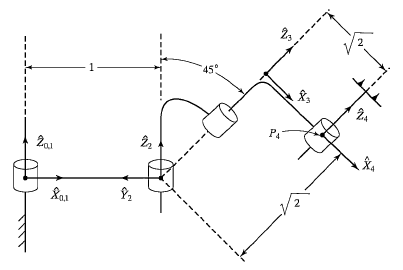
\includegraphics[]{Fig415}
\it{\caption{Schematic used for Exercise 4.17 (Figure 4.15) on page 131\cite{textbook}}}
\end{figure}
\subsubsection*{\textit{\textbf{Step 2: Fill the D-H Table}}}
\begin{center}
\begin{tabular}{ l | c c c c }
  $i$ & $\alpha_{i-1}$ & $a_{i-1}$ & $d_{i}$ & $\theta_{i}$ \\
  \hline
  1   & $0$            & $0$       & $0$     & $\theta_{1}$\\ 
  2   & $-90\degree$   & $1$       & $1$     & $\theta_{2}$\\
  3   & $45\degree$    & $0$       & $1$     & $\theta_{3}$\\
  4   & $0$            & $1$       & $0$     & $\theta_{4}$\\
\end{tabular}
\end{center}
\subsubsection*{\textit{\textbf{Step 3: }}$\bf{\it{\forall_{i}}}$ compute $\bf{\it{ \tensor*[^{i-1}_{i}]{T}{}}}$}
\[
\tensor*[^{0}_{1}]{T}{} =
\begin{bmatrix}
    c_{1}        & -s_{1}       & 0     & 0      \\
    s_{1}        & c_{1}        & 0     & 0      \\
    0            & 0            & 1     & 0      \\
    0            & 0            & 0     & 1
\end{bmatrix}, 
\tensor*[^{1}_{2}]{T}{} =
\begin{bmatrix}
    c_{2}        & -s_{2}       & 0     & 1      \\
    0            & 0            & 1     & 1      \\
    -s_{2}       & -c_{2}       & 0     & 0      \\
    0            & 0            & 0     & 1
\end{bmatrix}, 
\tensor*[^{2}_{3}]{T}{} =
\begin{bmatrix}
    c_{3}                            & -s_{3}                           & 0                       & 0  \\[6pt]
    \dfrac{\sqrt{2}}{2} s_{3}        & \dfrac{\sqrt{2}}{2} c_{3}        & -\dfrac{\sqrt{2}}{2}    & -\dfrac{\sqrt{2}}{2}      
    \\[6pt]
    -\dfrac{\sqrt{2}}{2} s_{3}       & \dfrac{\sqrt{2}}{2} c_{3}        & \dfrac{\sqrt{2}}{2}     & \dfrac{\sqrt{2}}{2}       
    \\[6pt]
    0                                & 0                                & 0                       & 1
\end{bmatrix}
\tensor*[^{3}_{4}]{T}{} =
\begin{bmatrix}
    c_{4}        & -s_{4}       & 0     & 1      \\
    s_{4}        & c_{4}        & 0     & 0      \\
    0            & 0            & 1     & 0      \\
    0            & 0            & 0     & 1
\end{bmatrix}\] \\
\subsubsection*{\textbf{\textit{Step 4: Find }}$\bf{\it{\tensor*[^{3}]{P}{_{4}}}}$, $\bf{\it{\tensor*[^{2}]{P}{_{4}}}}$,$\bf{\it{\tensor*[^{1}]{P}{_{4}}}}$,$\bf{\it{\tensor*[^{0}]{P}{_{4}}}}$}
\[
\tensor*[^{4}]{P}{_{4}} =
\begin{bmatrix}
   0 & 0 & 0 & 1
\end{bmatrix}^T
\]
\[
\tensor*[^{3}]{P}{_{4}} = \tensor*[^{3}_{4}]{T}{} \tensor*[^{4}]{P}{_{4}} =
\begin{bmatrix}
    c_{4}        & -s_{4}       & 0     & 1      \\
    s_{4}        & c_{4}        & 0     & 0      \\
    0            & 0            & 1     & 0      \\
    0            & 0            & 0     & 1
\end{bmatrix}
\begin{bmatrix}
   0 \\ 0 \\ 0 \\ 1
\end{bmatrix} =
\begin{bmatrix}
   1 \\ 0 \\ 0 \\ 1
\end{bmatrix}
\]
\[
\tensor*[^{2}]{P}{_{4}} = \tensor*[^{2}_{3}]{T}{} \tensor*[^{3}]{P}{_{4}} =
\begin{bmatrix}
    c_{3}                            & -s_{3}                           & 0                       & 0  \\[6pt]
    \dfrac{\sqrt{2}}{2} s_{3}        & \dfrac{\sqrt{2}}{2} c_{3}        & -\dfrac{\sqrt{2}}{2}    & -\dfrac{\sqrt{2}}{2}      \\[6pt]
    -\dfrac{\sqrt{2}}{2} s_{3}       & \dfrac{\sqrt{2}}{2} c_{3}        & \dfrac{\sqrt{2}}{2}     & \dfrac{\sqrt{2}}{2}       \\[6pt]
    0                                & 0                                & 0                       & 1
\end{bmatrix}
\begin{bmatrix}
   1 \\ 0 \\ 0 \\ 1
\end{bmatrix} =
\begin{bmatrix}
   c_{3} \\[6pt] \dfrac{\sqrt{2}}{2} s_{3} - \dfrac{\sqrt{2}}{2} \\[6pt] \dfrac{\sqrt{2}}{2} - \dfrac{\sqrt{2}}{2} s_{3} \\[6pt]  1
\end{bmatrix}
\]
\[
\tensor*[^{1}]{P}{_{4}} = \tensor*[^{1}_{2}]{T}{} \tensor*[^{2}]{P}{_{4}} =
\begin{bmatrix}
    c_{2}        & -s_{2}       & 0     & 1      \\
    0            & 0            & 1     & 1      \\
    -s_{2}       & -c_{2}       & 0     & 0      \\
    0            & 0            & 0     & 1
\end{bmatrix}
\begin{bmatrix}
   c_{3} \\[6pt] \dfrac{\sqrt{2}}{2} s_{3} - \dfrac{\sqrt{2}}{2} \\[6pt] \dfrac{\sqrt{2}}{2} - \dfrac{\sqrt{2}}{2} s_{3} \\[6pt]  1
\end{bmatrix} =
\begin{bmatrix}
    c_{23} + \dfrac{\sqrt{2}}{2}s_{3} - \dfrac{\sqrt{2}}{2} s_{23}  +  1        \\[6pt]
    \dfrac{\sqrt{2}}{2} - \dfrac{\sqrt{2}}{2} s_{3} +  1                        \\[6pt]
    \dfrac{\sqrt{2}}{2}c_{2} - s_{2}c_{3} - \dfrac{\sqrt{2}}{2}c_{2}s_{3}       \\[6pt]
    1
\end{bmatrix}
\]
\[
\tensor*[^{0}]{P}{_{4}} = \tensor*[^{0}_{1}]{T}{} \tensor*[^{1}]{P}{_{4}} =
\begin{bmatrix}
    c_{1}        & -s_{1}       & 0     & 0      \\
    s_{1}        & c_{1}        & 0     & 0      \\
    0            & 0            & 1     & 0      \\
    0            & 0            & 0     & 1
\end{bmatrix}
\begin{bmatrix}
    c_{23} + \dfrac{\sqrt{2}}{2}s_{3} - \dfrac{\sqrt{2}}{2} s_{23}  +  1        
    \\[6pt]
    \dfrac{\sqrt{2}}{2} - \dfrac{\sqrt{2}}{2} s_{3} +  1                        
    \\[6pt]
    \dfrac{\sqrt{2}}{2}c_{2} - s_{2}c_{3} - \dfrac{\sqrt{2}}{2}c_{2}s_{3}       
    \\[6pt]
    1
\end{bmatrix} 
\]
\[
\tensor*[^{0}]{P}{_{4}} =
\begin{bmatrix}
   c_{123} + \dfrac{\sqrt{2}}{2}c_{1}s_{3} - \dfrac{\sqrt{2}}{2}c_{1}s_{23}  +  c_{1} - \dfrac{\sqrt{2}}{2}s_{1} + \dfrac{\sqrt{2}}{2} s_{13} -  s_{1} 
   \\[6pt]
   s_{1}c_{23} + \dfrac{\sqrt{2}}{2}s_{13} - \dfrac{\sqrt{2}}{2} s_{123}  +  s_{1} - \dfrac{\sqrt{2}}{2}c_{2} + \dfrac{\sqrt{2}}{2}c_{2}s_{3} - c_{2} 
   \\[6pt]
   \dfrac{\sqrt{2}}{2}c_{2} - s_{2}c_{3} - \dfrac{\sqrt{2}}{2}c_{2}s_{3} 
   \\[6pt]
   1
\end{bmatrix}
\]
\subsubsection*{\textbf{\textit{Step 5: Find }}$\bf{\it{\theta_{3}}}$}
An order to compute $\theta_{3}$, we can equate the following:
\[
\tensor*[^{0}]{P}{_{4}} =
\begin{bmatrix}
   c_{123} + \dfrac{\sqrt{2}}{2}c_{1}s_{3} - \dfrac{\sqrt{2}}{2}c_{1}s_{23}  +  c_{1} - \dfrac{\sqrt{2}}{2}s_{1} + \dfrac{\sqrt{2}}{2} s_{13} -  s_{1} 
   \\[6pt]
   s_{1}c_{23} + \dfrac{\sqrt{2}}{2}s_{13} - \dfrac{\sqrt{2}}{2} s_{123}  +  s_{1} - \dfrac{\sqrt{2}}{2}c_{2} + \dfrac{\sqrt{2}}{2}c_{2}s_{3} - c_{2} 
   \\[6pt]
   \dfrac{\sqrt{2}}{2}c_{2} - s_{2}c_{3} - \dfrac{\sqrt{2}}{2}c_{2}s_{3} 
   \\[6pt]
   1
\end{bmatrix} = 
\begin{bmatrix}
   x\\[6pt]
   y\\[6pt]
   z\\[6pt]
   1
\end{bmatrix}
\]
Now, we let $\theta_{1}$ and $\theta_{2}$ equal 0, producing:
\[
y = -\dfrac{\sqrt{2}}{2}+\dfrac{\sqrt{2}}{2}s_{3} - 1
\mbox{    }\Rightarrow\mbox{    }
s_{3} = \dfrac{2y + 2\sqrt{2} + 2}{\sqrt{2}},
\mbox{                }
z = \dfrac{\sqrt{2}}{2} - \dfrac{\sqrt{2}}{2}s_{3}
\mbox{    }\Rightarrow\mbox{    }
c_{3} = 1 - \dfrac{2z\sqrt{2}}{2}
\]
Then we can do the following to get $\theta_{3}$:
\[
\theta_{3} = tan^{-1}\dfrac{s_{3}}{c_{3}}
\]
When we plug in our point values from above ($\tensor*[^{0}]{P}{_{4ORG}} = [0.0, 1.0, 1.414]^T$), we get the following:
\[
\theta_{3} = tan^{-1}\dfrac{4.83}{3} \approx \pm 60\degree
\]
\section*{Problem 5}
\subsection*{Exercise 5.1}
Repeat Example 5.3, but using the Jacobian written in frame \{0\}. Are the results the same as those of Example 5.3?
\subsubsection*{\textit{\textbf{Step 1: Assign Frames}}}
\begin{figure}[!h]
\centering
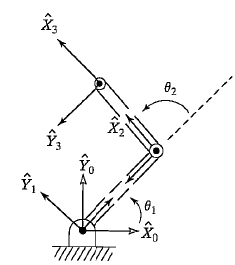
\includegraphics[]{Fig59}
\it{\caption{Frame assignment for Figure 5.9 (Example 5.3) on page 147\cite{textbook}}}
\end{figure}
\subsubsection*{\textit{\textbf{Step 2: Fill the D-H Table}}}
\begin{center}
\begin{tabular}{ l | c c c c }
  $i$ & $\alpha_{i-1}$ & $a_{i-1}$ & $d_{i}$ & $\theta_{i}$ \\
  \hline
  1   & $0$            & $0$       & $0$     & $\theta_{1}$\\ 
  2   & $0$    		   & $l_{1}$   & $0$     & $\theta_{2}$\\
  3   & $0$    		   & $l_{2}$   & $0$     & $0$
\end{tabular}
\end{center}
\subsubsection*{\textit{\textbf{Step 3: }}$\bf{\it{\forall_{i}}}$ compute $\bf{\it{ \tensor*[^{i-1}_{i}]{T}{}}}$}
%%%%%%%%%%%%%%%%%%%%% BEGIN INITIAL SETUP %%%%%%%%%%%%%%%%%%%%%%%%%%%%%%%%%%%%%%%%%%
\[
\tensor*[^{0}_{1}]{T}{} =
\begin{bmatrix}
    c_{1}        & -s_{1}       & 0     & 0      \\
    s_{1}        & c_{1}        & 0     & 0      \\
    0            & 0            & 1     & 0      \\
    0            & 0            & 0     & 1
\end{bmatrix}, 
\tensor*[^{1}_{2}]{T}{} =
\begin{bmatrix}
    c_{2}        & -s_{2}       & 0     & l_{1}      \\
    s_{2}        & c_{2}        & 0     & 0      \\
    0            & 0            & 1     & 0      \\
    0            & 0            & 0     & 1
\end{bmatrix}, 
\tensor*[^{2}_{3}]{T}{} =
\begin{bmatrix}
    1            & 0            & 0     & l_{2}  \\
    0            & 1            & 0     & 0      \\
    0            & 0            & 1     & 0      \\
    0            & 0            & 0     & 1
\end{bmatrix}\] \\
\subsubsection*{\textit{\textbf{Step 3: Compute Jacobian}}}
\[
\tensor*[^{3}_{0}]{R}{} =
\tensor*[^{3}_{2}]{R}{}
\tensor*[^{2}_{1}]{R}{}
\tensor*[^{1}_{0}]{R}{} =
\begin{bmatrix}
    c_{12} - s_{12}  		& -s_{1}c_{2} - c_{1}s_{2}  & 0     \\
    c_{1}s_{2} + s_{1}c_{2} & c_{12} - s_{12}       	& 0     \\
    0            			& 0        					& 1     
\end{bmatrix}
\]
\[
\tensor*[^{3}]{v}{_0} =
\tensor*[^{3}_{0}]{R}{}\tensor*[^{3}]{v}{_3}=
\begin{bmatrix}
    c_{12} - s_{12}  		& -s_{1}c_{2} - c_{1}s_{2}  & 0     \\
    c_{1}s_{2} + s_{1}c_{2} & c_{12} - s_{12}       	& 0     \\
    0            			& 0        					& 1     
\end{bmatrix}
\begin{bmatrix}
    l_{1}s_{2}\dot{\theta_{1}}    		  \\
    l_{1}c_{2}\dot{\theta_{1}} + l_{2}(\dot{\theta_{1}} + \dot{\theta_{2}})    \\
    0   
\end{bmatrix}
\]
\[
\tensor*[^{3}]{v}{_3} =
\begin{bmatrix}
    l_{1}s_{2}\dot{\theta_{1}}(c_{12} - s_{12}) + (l_{1}c_{2}\dot{\theta_{1}} + l_{2}(\dot{\theta_{1}} + \dot{\theta_{2}}))(-s_{1}c_{2} - c_{1}s_{2})  		  \\
    l_{1}s_{2}\dot{\theta_{1}}(c_{1}s_{2} + s_{1}c_{2}) + (l_{1}c_{2}\dot{\theta_{1}} + l_{2}(\dot{\theta_{1}} + \dot{\theta_{2}}))(c_{12} - s_{12})    \\
    0   
\end{bmatrix}
\]\\
The results are not the same as those of Example 5.3, which is expected since we are computed the Jacobian from the opposite end frame.  Forces are applied differently depending on the frame selected.
\subsection*{Exercise 5.2}
Find the Jacobian of the manipulator with three degrees of freedom from Exercise 3 of Chapter 3. Write it in terms of a frame \{4\} located at the tip of the hand and having the same orientation as frame \{3\}.
\subsubsection*{\textit{\textbf{Step 1: Assign Frames}}}
\begin{figure}[!h]
\centering
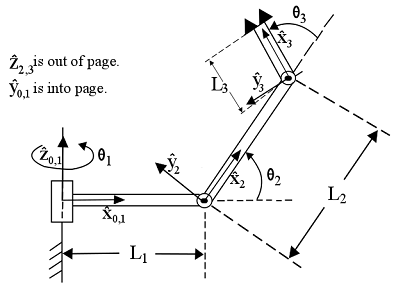
\includegraphics[]{Fig329b}
\it{\caption{Frame assignment for Figure 3.29 (Exercise 3.3) on page 93\cite{textbook}}}
\end{figure}
\subsubsection*{\textit{\textbf{Step 2: Fill the D-H Table}}}
\begin{center}
\begin{tabular}{ l | c c c c }
  $i$ & $\alpha_{i-1}$ & $a_{i-1}$ & $d_{i}$ & $\theta_{i}$ \\
  \hline
  1   & $0$            & $0$       & $0$     & $\theta_{1}$\\ 
  2   & $90\degree$    & $L_{1}$   & $0$     & $\theta_{2}$\\
  3   & $0$            & $L_{2}$   & $0$     & $\theta_{3}$\\
  4   & $0$            & $L_{3}$   & $0$     & $0$
\end{tabular}
\end{center}
\subsubsection*{\textit{\textbf{Step 3: }}$\bf{\it{\forall_{i}}}$ compute $\bf{\it{ \tensor*[^{i-1}_{i}]{T}{}}}$}
%%%%%%%%%%%%%%%%%%%%% BEGIN INITIAL SETUP %%%%%%%%%%%%%%%%%%%%%%%%%%%%%%%%%%%%%%%%%%
\[
\tensor*[^{0}_{1}]{T}{} =
\begin{bmatrix}
    c_{1}        & -s_{1}       & 0     & 0      \\
    s_{1}        & c_{1}        & 0     & 0      \\
    0            & 0            & 1     & 0      \\
    0            & 0            & 0     & 1
\end{bmatrix}, 
\tensor*[^{1}_{2}]{T}{} =
\begin{bmatrix}
    c_{2}        & -s_{2}       & 0     & L_{1}  \\
    0            & 0            & -1    & 0      \\
    s_{2}        & c_{2}        & 0     & 0      \\
    0            & 0            & 0     & 1
\end{bmatrix}, 
\tensor*[^{2}_{3}]{T}{} =
\begin{bmatrix}
    c_{3}        & -s_{3}       & 0     & L_{2}  \\
    s_{3}        & c_{3}        & 0     & 0      \\
    0            & 0            & 1     & 0      \\
    0            & 0            & 0     & 1
\end{bmatrix},
\tensor*[^{3}_{4}]{T}{} =
\begin{bmatrix}
    1            & 0            & 0     & L_{3}  \\
    0            & 1            & 0     & 0      \\
    0            & 0            & 1     & 0      \\
    0            & 0            & 0     & 1
\end{bmatrix}\] \\
%%%%%%%%%%%%%%%%%%%%% COMPUTE 0 to 2 %%%%%%%%%%%%%%%%%%%%%%%%%%%%%%%%%%%%%%%%%%
\[
\tensor*[^{0}_{2}]{T}{} = 
\tensor*[^{0}_{1}]{T}{} \tensor*[^{1}_{2}]{T}{} = 
\begin{bmatrix}
    c_{12}       & -c_{1}s_{2}  & s_{1} & c_{1}L_{1}     \\
    s_{1}c_{2}   & -s_{12}      & -c_{1}& s_{1}L_{1}     \\
    s_{2}        & c_{2}        & 0     & 0      \\
    0            & 0            & 0     & 1
\end{bmatrix}
\] \\
%%%%%%%%%%%%%%%%%%%%% COMPUTE 0 to 3 %%%%%%%%%%%%%%%%%%%%%%%%%%%%%%%%%%%%%%%%%%
\[
\tensor*[^{0}_{3}]{T}{} = 
\tensor*[^{0}_{2}]{T}{} \tensor*[^{2}_{3}]{T}{} =
\begin{bmatrix}
c_{123}-c_{1}s_{2,3}   & -c_{12}s_{3}-c_{13}s_{2} & s_{1} & c_{1}L_{1} + c_{12}L_{2}\\
s_{1}c_{23}-s_{123}    & -s_{13}c_{2}-s_{12}c_{3} & -c_{1}& s_{1}L_{1} + s_{1}c_{2}L_{2}\\
s_{2}c_{3}+c_{2}s_{3}  & c_{23}-s_{23}            & 0     & s_{2}L_{2}\\
0                      & 0                        & 0     & 1
\end{bmatrix}
\]
%%%%%%%%%%%%%%%%%%%% COMPUTE 0 to 4 %%%%%%%%%%%%%%%%%%%%%%%%%%%%%%%%%%%%%%%%%%%
\[
\tensor*[^{0}_{4}]{T}{} =
\tensor*[^{0}_{3}]{T}{} \tensor*[^{3}_{4}]{T}{} 
\begin{bmatrix}
c_{123}-c_{1}s_{2,3}   & -c_{12}s_{3}-c_{13}s_{2} & s_{1} & c_{1}L_{1} + c_{12}L_{2}\\
s_{1}c_{23}-s_{123}    & -s_{13}c_{2}-s_{12}c_{3} & -c_{1}& s_{1}L_{1} + s_{1}c_{2}L_{2}\\
s_{2}c_{3}+c_{2}s_{3}  & c_{23}-s_{23}            & 0     & s_{2}L_{2}\\
0                      & 0                        & 0     & 1
\end{bmatrix}
\begin{bmatrix}
1    & 0    & 0     & L_{3}  \\
0    & 1    & 0     & 0      \\
0    & 0    & 1     & 0      \\
0    & 0    & 0     & 1
\end{bmatrix}
\]
\[
\tensor*[^{0}_{4}]{T}{} =
\begin{bmatrix}
c_{123}-c_{1}s_{2,3}   & -c_{12}s_{3}-c_{13}s_{2} & s_{1} & c_{123}L_{3} - c_{1}s_{2,3}L_{3} + c_{1}L_{1} + c_{12}L_{2}\\
s_{1}c_{23}-s_{123}    & -s_{13}c_{2}-s_{12}c_{3} & -c_{1}& s_{1}c_{23}L_{3} - s_{123}L_{3} + s_{1}L_{1} + s_{1}c_{2}L_{2}\\
s_{2}c_{3}+c_{2}s_{3}  & c_{23}-s_{23}            & 0     & s_{2}c_{3}L_{3} + c_{2}s_{3}L_{3} + s_{2}L_{2}\\
0                      & 0                        & 0     & 1
\end{bmatrix}
\]
%%%%%%%%%%%%%%%%%%%%%%%%%%%%%%% COMPLETED AND CORRECT %%%%%%%%%%%%%%%%%%%%%%%%%%%%
\subsubsection*{\textbf{\textit{Step 4: Compute Jacobian}}}
\[
\tensor*[^{0}_{4}]{R}{} =
\begin{bmatrix}
c_{123}-c_{1}s_{2,3}   & -c_{12}s_{3}-c_{13}s_{2} & s_{1} \\
s_{1}c_{23}-s_{123}    & -s_{13}c_{2}-s_{12}c_{3} & -c_{1}\\
s_{2}c_{3}+c_{2}s_{3}  & c_{23}-s_{23}            & 0      
\end{bmatrix}
\]
\[
\tensor*[^{1}]{\omega}{_1} =
\begin{bmatrix}
0 \\
0 \\
\dot{\theta_{1}}   
\end{bmatrix},
\tensor*[^{2}]{\omega}{_2} =
\begin{bmatrix}
0 \\
0 \\
\dot{\theta_{1}} + \dot{\theta_{2}} 
\end{bmatrix},
\tensor*[^{2}]{\omega}{_2} =
\begin{bmatrix}
0 \\
\dot{\theta_{2}} \\
\dot{\theta_{1}}  
\end{bmatrix},
\tensor*[^{3}]{\omega}{_3} =
\begin{bmatrix}
0 \\
\dot{\theta_{2}} + \dot{\theta_{3}} \\
\dot{\theta_{1}}  
\end{bmatrix},
\tensor*[^{4}]{\omega}{_4} =
\begin{bmatrix}
0 \\
\dot{\theta_{2}} + \dot{\theta_{3}} \\
\dot{\theta_{1}}  
\end{bmatrix}
\]
\[
\tensor*[^{1}]{v}{_1} =
\begin{bmatrix}
0 \\
0 \\
0 
\end{bmatrix},
\tensor*[^{2}]{v}{_2} =
\begin{bmatrix}
    c_{2}        & -s_{2}       & 0    \\
    0            & 0            & -1   \\
    s_{2}        & c_{2}        & 0
\end{bmatrix}
\begin{bmatrix}
l_1\dot{\theta_{1}}\\
0 \\
0 
\end{bmatrix} =
\begin{bmatrix}
    c_{2}l_1\dot{\theta_{1}}   \\
    0  \\
    s_{2}l_1\dot{\theta_{1}}
\end{bmatrix}
,
\tensor*[^{3}]{v}{_3} =
\begin{bmatrix}
    c_{3}        & -s_{3}       & 0     \\
    s_{3}        & c_{3}        & 0     \\
    0            & 0            & 1 
\end{bmatrix}
\begin{bmatrix}
    c_{2}l_1\dot{\theta_{1}}   \\
    0  \\
    s_{2}l_1\dot{\theta_{1}}
\end{bmatrix} = 
\begin{bmatrix}
    c_{23}l_1\dot{\theta_{1}}   \\
    c_{2}s_{3}l_1\dot{\theta_{1}} \\
    s_{2}l_1\dot{\theta_{1}}
\end{bmatrix}
= \tensor*[^{4}]{v}{_4}
\]
\[
\tensor*[^{0}_{4}]{R}{}
\tensor*[^{4}]{v}{_4} =
\begin{bmatrix}
c_{123}-c_{1}s_{23}   & -c_{12}s_{3}-c_{13}s_{2} & s_{1} \\
s_{1}c_{23}-s_{123}    & -s_{13}c_{2}-s_{12}c_{3} & -c_{1}\\
s_{2}c_{3}+c_{2}s_{3}  & c_{23}-s_{23}            & 0      
\end{bmatrix}
\begin{bmatrix}
    c_{23}l_1\dot{\theta_{1}}   \\
    c_{2}s_{3}l_1\dot{\theta_{1}} \\
    s_{2}l_1\dot{\theta_{1}}
\end{bmatrix} 
\]
\[
\tensor*[^{0}]{v}{_4} =
\begin{bmatrix}
(c_{123}-c_{1}s_{23})c_{23}l_1\dot{\theta_{1}} + 
(-c_{12}s_{3}-c_{13}s_{2})c_{2}s_{3}l_1\dot{\theta_{1}} +
s_{12}l_1\dot{\theta_{1}} \\
(s_{1}c_{23}-s_{123})c_{2}s_{3}l_1\dot{\theta_{1}} +
(-s_{13}c_{2}-s_{12}c_{3})c_{2}s_{3}l_1\dot{\theta_{1}} +
(-c_{1}s_{2}l_1\dot{\theta_{1}}) \\
(s_{2}c_{3}+c_{2}s_{3})c_{23}l_1\dot{\theta_{1}} + (c_{23}-s_{23})c_{2}s_{3}l_1\dot{\theta_{1}}
\end{bmatrix}
\]
%%%%%%%%%%%%%%%%%%%%%%%%%%%%%%%%%%%%%%%%%%%%%%%%%%%%%%%%%%%%%%%%%%%%%%%%%%%%%%%%
%%%%%%%%%%%%%%%%%%%%%%%%%%%%%%%%%REFERENCES%%%%%%%%%%%%%%%%%%%%%%%%%%%%%%%%%%%%%
\bibliographystyle{IEEEtran}
\bibliography{IEEEabrv,project}
\end{document}
